\section{Coverage Methodology and Results}
\label{sec:coverage_methodology}

Coverage was treated not as a target to be gamed but as a diagnostic: a way to find branches that no test exercised and to decide, branch by branch, whether the gap represented a real risk worth closing.

\subsection{Measurement Workflow}

Coverage is collected with Go's built-in tooling \cite{go_testing}. The whole module is tested with statement-coverage instrumentation, and the resulting profile is summarized per function:

\begin{verbatim}
go test ./... -coverprofile=coverage.out -count=1
go tool cover -func=coverage.out
\end{verbatim}

The \texttt{-count=1} flag disables the test cache so that every run is fresh. The per-function summary from \texttt{go tool cover -func} drives a \textbf{gap-analysis loop}: functions below full coverage are inspected to identify which branches are unexercised --- typically validation failures, error returns, and edge inputs --- and a targeted test is then written for each genuinely reachable gap. \texttt{go tool cover -html} was used during development to visualize uncovered lines directly in source. Over the most recent round this loop raised overall statement coverage from a \textbf{75.5\%} baseline to \textbf{79.3\%}.

\subsection{Per-Component Results}

Table~\ref{tab:coverage_results} reports statement coverage per package from the most recent \texttt{go tool cover -func} run. Packages whose responsibility is pure logic --- models, configuration, middleware, and response helpers --- reach 100\%, while packages that wrap external systems settle in the high-80s to low-90s, where the remaining gaps are defensive or unreachable branches discussed in Section~\ref{sec:testing_limitations}.

\begin{table}[H]
    \centering
    \renewcommand{\arraystretch}{1.2}
    \begin{tabular}{lc}
    \toprule
    \textbf{Package} & \textbf{Statement Coverage} \\
    \midrule
    \texttt{internal/config}              & 100.0\% \\
    \texttt{internal/middleware}          & 100.0\% \\
    \texttt{internal/model}               & 100.0\% \\
    \texttt{internal/response}            & 100.0\% \\
    \texttt{internal/mongodb/handler}     & 100.0\% \\
    \texttt{internal/mongodb/route}       & 100.0\% \\
    \texttt{internal/postgres/route}      & 100.0\% \\
    \texttt{internal/postgres/repository} & 99.6\% \\
    \texttt{internal/route}               & 97.8\% \\
    \texttt{internal/handler}             & 96.8\% \\
    \texttt{internal/postgres/handler}    & 94.1\% \\
    \texttt{internal/utils}               & 93.7\% \\
    \texttt{internal/postgres/service}    & 90.2\% \\
    \texttt{internal/mongodb/infra}       & 90.1\% \\
    \texttt{internal/mongodb/service}     & 90.0\% \\
    \texttt{internal/backup}              & 88.9\% \\
    \texttt{internal/repository}          & 85.8\% \\
    \texttt{internal/service}             & 82.5\% \\
    \midrule
    \textbf{Overall (module)}             & \textbf{79.3\%} \\
    \bottomrule
    \end{tabular}
    \caption{Per-package statement coverage and overall module figure}
    \label{tab:coverage_results}
\end{table}

The overall module figure (79.3\%) is lower than any tested package because the module also contains entrypoint and wiring packages --- \texttt{cmd/api}, \texttt{cmd/pgproxy}, \texttt{internal/server}, and infrastructure adapters --- that contain only bootstrapping code and carry no unit tests by design. Their statements dilute the aggregate without representing untested business logic.

The gap-analysis loop produced concrete, measurable improvements in the packages that wrap external systems. Notable examples include the MongoDB collection service, raised from \textbf{32.5\%} to roughly \textbf{90\%}; the PostgreSQL Schema-AI SSE proxy in \texttt{schema\_handler.go}, raised from \textbf{0\%} to about \textbf{86\%} with its stream handler reaching \textbf{100\%}; the index operations in \texttt{table\_service\_indexes.go} at \textbf{100\%}; and \texttt{user\_handler.go} at \textbf{100\%} with every reachable branch of \texttt{project\_handler.go} covered. The Google authentication service's constructor reached \textbf{100\%} and its \texttt{Callback} \textbf{93.3\%}, while \texttt{FetchUserInfo} remained partial for the reasons given in Section~\ref{sec:testing_limitations}. Figure~\ref{fig:coverage_improvement} visualizes the two most dramatic of these jumps alongside the movement in the overall module figure.

\begin{figure}[H]
    \centering
    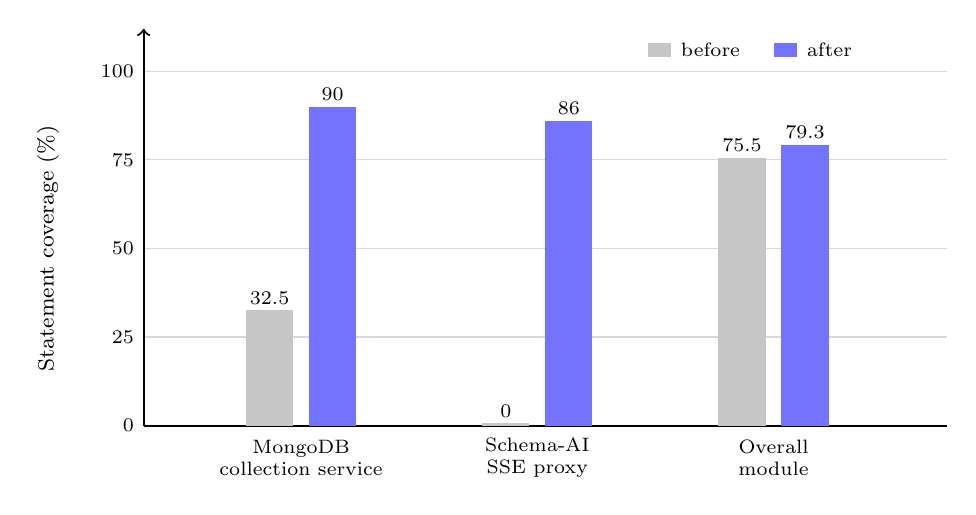
\begin{tikzpicture}[y=0.045cm, x=1cm]
        % --- axes and gridlines (0..100 mapped via y=0.045cm) ---
        \foreach \v in {0,25,50,75,100} {
            \draw[gray!30] (0,\v) -- (10.2,\v);
            \node[left, font=\scriptsize] at (0,\v) {\v};
        }
        \draw[->, thick] (0,0) -- (0,112);
        \draw[thick] (0,0) -- (10.2,0);
        \node[rotate=90, font=\footnotesize, anchor=south] at (-0.95,50) {Statement coverage (\%)};

        % --- helper: groups centered at x = 2, 5, 8 ---
        % before bar = gray, after bar = blue
        % Group 1: MongoDB collection service 32.5 -> 90
        \fill[gray!45]  (1.3,0) rectangle (1.9,32.5);
        \fill[blue!55]  (2.1,0) rectangle (2.7,90);
        \node[font=\scriptsize] at (1.6,36)  {32.5};
        \node[font=\scriptsize] at (2.4,93.5) {90};
        \node[align=center, font=\scriptsize, text width=2.6cm] at (2.0,-9) {MongoDB\\collection service};

        % Group 2: Schema-AI SSE proxy 0 -> 86
        \fill[gray!45]  (4.3,0) rectangle (4.9,0.6);
        \fill[blue!55]  (5.1,0) rectangle (5.7,86);
        \node[font=\scriptsize] at (4.6,4)    {0};
        \node[font=\scriptsize] at (5.4,89.5)  {86};
        \node[align=center, font=\scriptsize, text width=2.6cm] at (5.0,-9) {Schema-AI\\SSE proxy};

        % Group 3: Overall module 75.5 -> 79.3
        \fill[gray!45]  (7.3,0) rectangle (7.9,75.5);
        \fill[blue!55]  (8.1,0) rectangle (8.7,79.3);
        \node[font=\scriptsize] at (7.6,79)    {75.5};
        \node[font=\scriptsize] at (8.4,82.8)   {79.3};
        \node[align=center, font=\scriptsize, text width=2.6cm] at (8.0,-9) {Overall\\module};

        % --- legend ---
        \fill[gray!45] (6.4,104) rectangle (6.7,108);
        \node[right, font=\scriptsize] at (6.7,106) {before};
        \fill[blue!55] (8.0,104) rectangle (8.3,108);
        \node[right, font=\scriptsize] at (8.3,106) {after};
    \end{tikzpicture}
    \caption{Statement coverage before and after the gap-analysis loop for the two most affected components and for the overall module.}
    \label{fig:coverage_improvement}
\end{figure}
